\section{A Graphical Program Representation}
\label{sec:graph-representation}

This section presents \programl, a novel IR-based program representation that
closely matches the data structures used traditionally in inter-procedural data
flow analysis and can be processed natively by deep learning models. We
represent programs as directed multigraphs where instructions, variables, and
constants are vertices, and relations between vertices are edges. Edges are
typed to differentiate control-, \mbox{data-,} and call-flow. Additionally, we
augment edges with a local position attribute to encode the order of operands to
instructions, and to differentiate between divergent branches in control-flow.

\begin{figure*}[t]
  \centering %
  \begin{subfigure}[t]{.46\linewidth}%
  	\centering
  	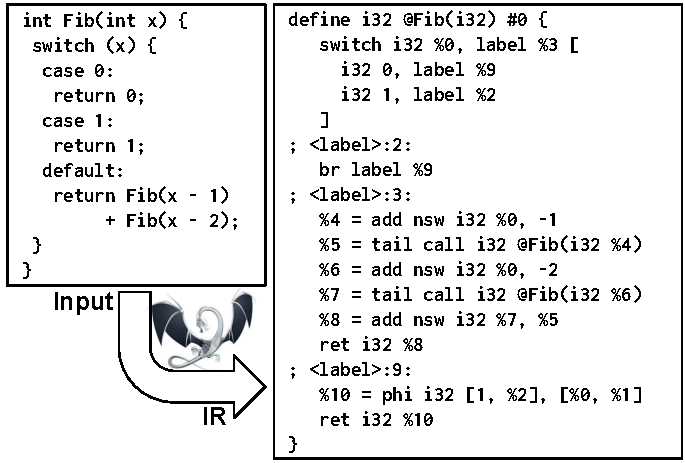
\includegraphics[width=.95\linewidth]{images/A_IR}%
    \captionsetup{width=.95\linewidth}%
  	\caption{%
      The input program is passed through the compiler front-end to produce an
      IR. In this example, LLVM-IR is used.%
    }
  	\label{subfigure:ir}%
  \end{subfigure}
  \quad
	\begin{subfigure}[t]{.46\linewidth}%
		\centering
  	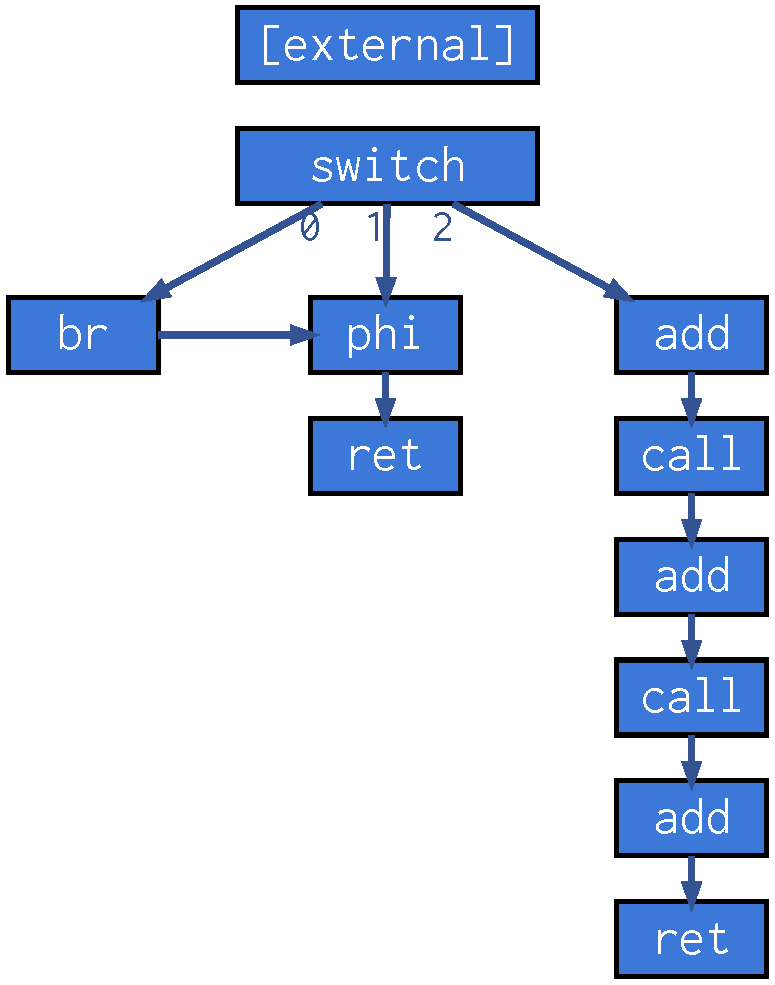
\includegraphics[width=.51\linewidth]{images/B_Control}%
    \captionsetup{width=.95\linewidth}%
  	\caption{%
      A full-flow graph is constructed of instructions and control dependencies.
      All edges have position attributes; for clarity, we have omitted position
      labels where not required.%
    }
  	\label{subfigure:control_flow}%
	\end{subfigure}
  \\*
  \begin{subfigure}[t]{.46\linewidth}%
  	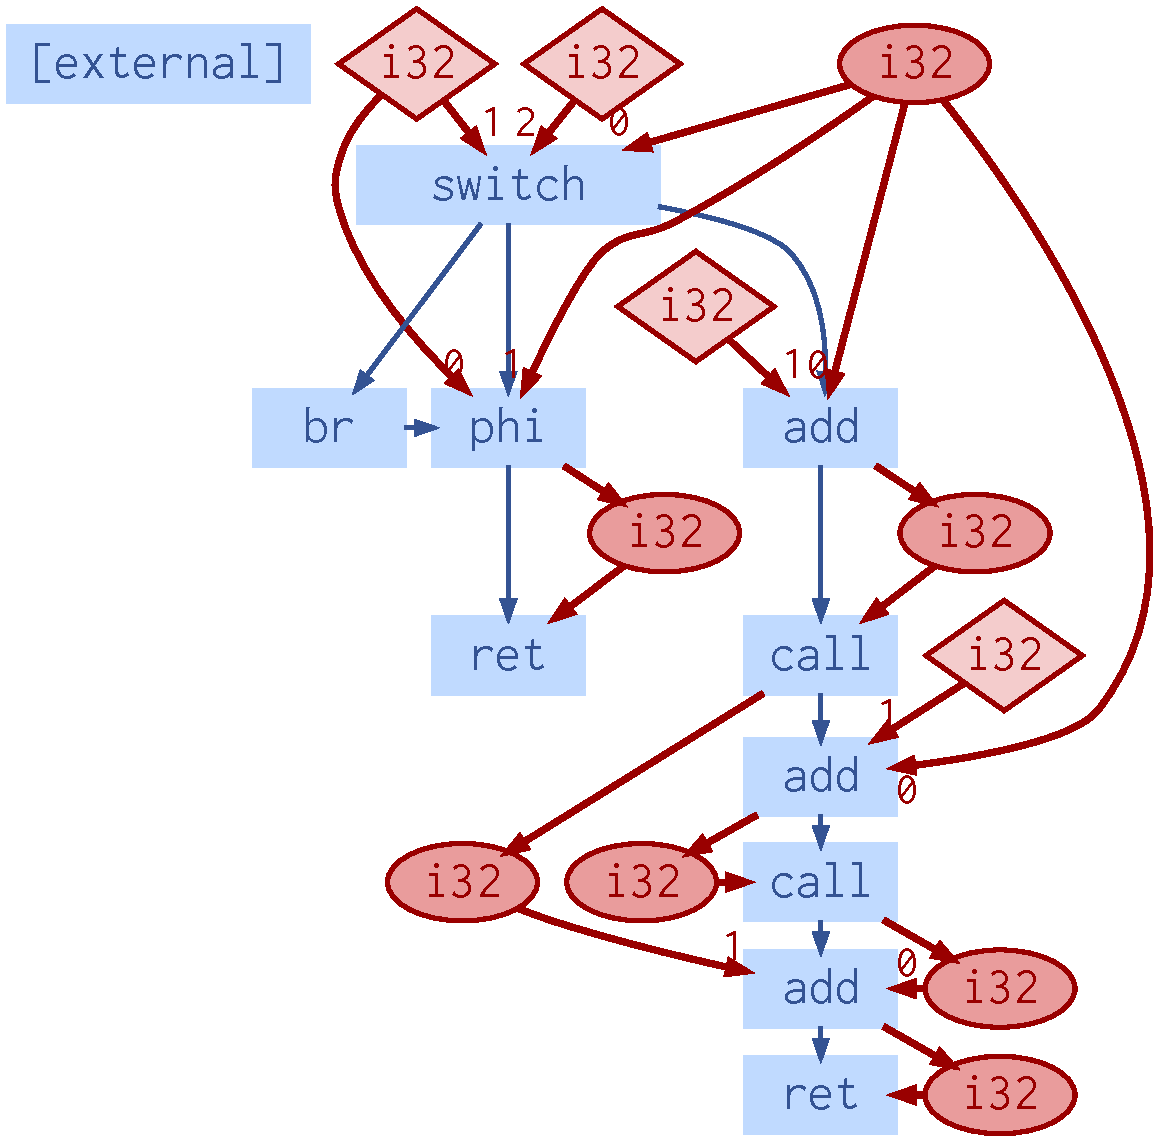
\includegraphics[width=.72\linewidth]{images/C_Data}%
    \captionsetup{width=.95\linewidth}%
  	\caption{%
      Vertices are added for data elements (elliptical nodes are variables,
      diamonds are constants). Data edges capture use/def relations.
      \texttt{i32} indicates 32 bit signed integers. Numbers on edges indicate
      operand positions.} \label{subfigure:data_flow}%
	\end{subfigure}
	\quad
  \begin{subfigure}[t]{.46\linewidth}%
	  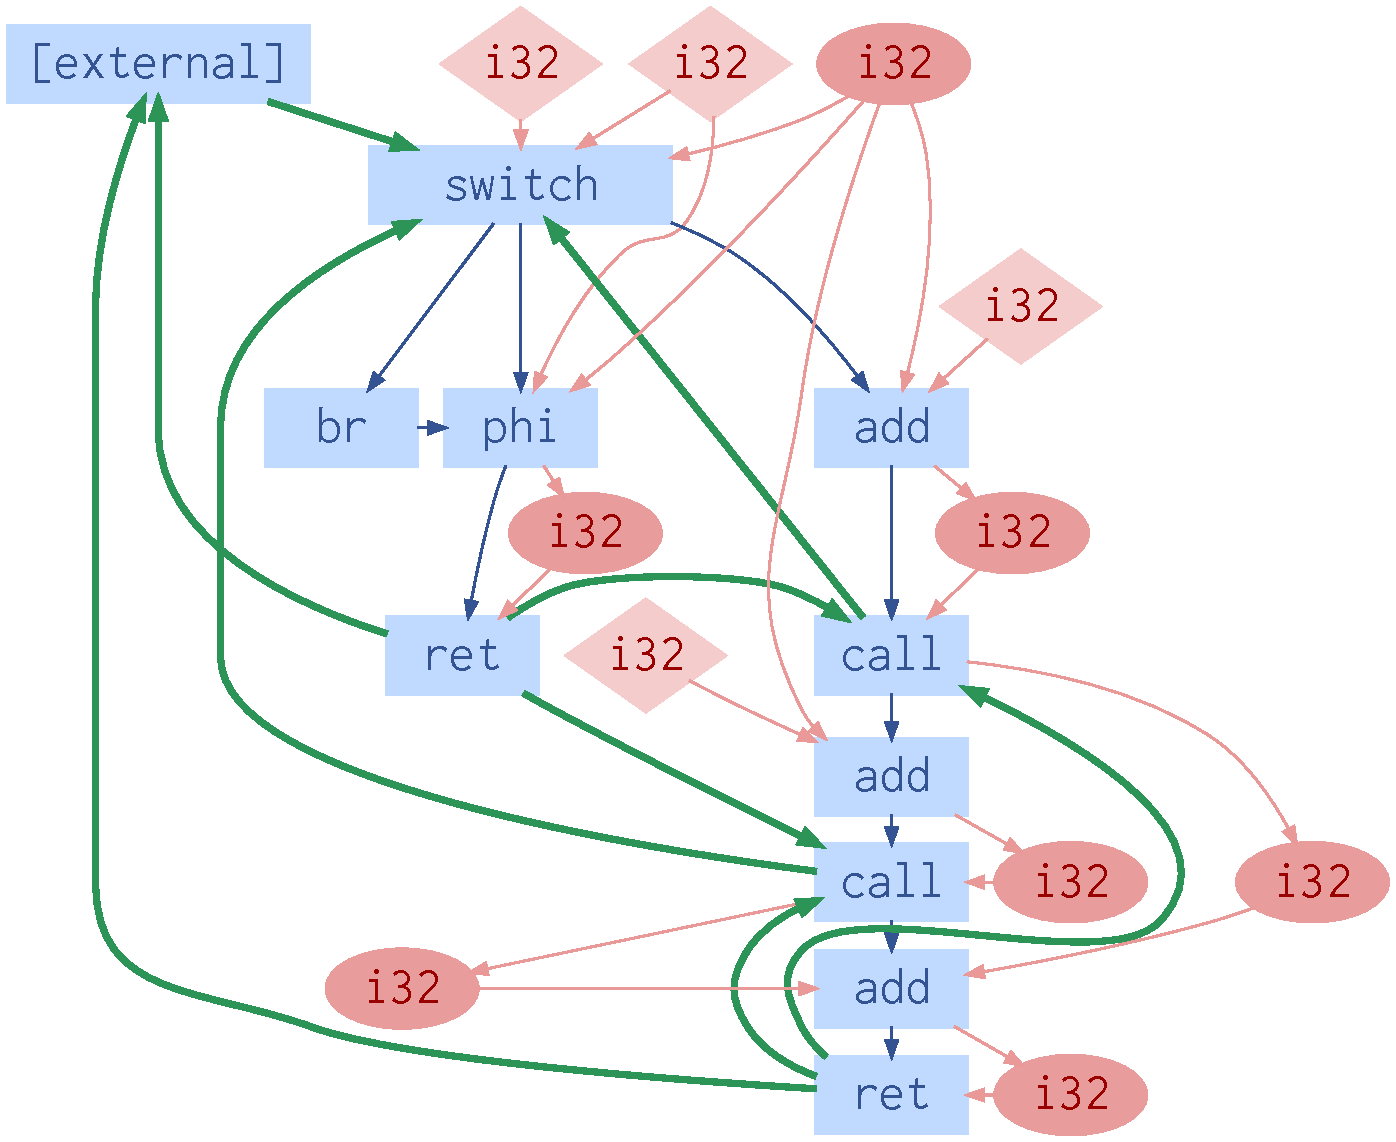
\includegraphics[width=.85\linewidth]{images/D_Call}%
    \captionsetup{width=.95\linewidth}%
	  \caption{%
      Functions have a single entry instruction and zero or more exit
      instructions. Call edges are inserted from call sites to function entry
      instructions, and return-edges from function exits to call sites.%
    }
	  \label{subfigure:call_flow}%
	\end{subfigure}
  \caption{%
    \programl construction from a Fibonacci sequence implementation using
    LLVM-IR.%
  }%
  \label{figure:graph_construction}%
  \vspace{-1em}
\end{figure*}

We construct a \programl graph $G = (V, E)$ by traversing a compiler IR. An
initially empty graph $G = \emptyset$ is populated in three stages:
control-flow, data-flow, and call-flow, shown in
Figure~\ref{figure:graph_construction}. In practice the three stages of graph
construction can be combined in a single $\bigo{(|V|+|E|)}$ pass.

\paragraph{(I) Control Flow} We construct the full-flow graph of an IR by
inserting a vertex for each instruction and connecting control-flow edges
(Fig.~\ref{subfigure:ir}, \ref{subfigure:control_flow}). Control edges are
augmented with numeric positions using an ascending sequence based on their
order in an instruction's successors.

\paragraph{(II) Data Flow} We introduce constant values and variables as graph
vertices (Fig.~\ref{subfigure:data_flow}). Data-flow edges are inserted to
capture the relation from constants and variables to the instructions that use
them as operands, and from instructions to produced variables. As each unique
variable and constant is a vertex, variables can be distinguished by their
scope, and unlike the source-level representations of prior works, variables in
different scopes map to distinct vertices and can thus be discerned. Data edges
have a position attribute that encodes the order of operands for instructions.
The latent representation of a statement (e.g., \texttt{\%1 = add i32 \%0, 1})
is thus a function of the vertex representing the instruction and the vertices
of any operand variables or constants, modulated by their order in the list of
operands.

\paragraph{(III) Call Flow} Call edges capture the relation between an
instruction that calls a function and the entry instruction of the called
function (Fig.~\ref{subfigure:call_flow}). Return call edges are added from each
of the terminal instructions of a function to the calling statement. Control
edges do not span functions, such that an IR with functions $F$ produces $|F|$
disconnected subgraphs (the same is not true for data edges which may cross
function boundaries, e.g., in the case of a global constant which is used across
many parts of a program). For IRs that support external linkage, an additional
vertex is created representing an external call site and connected to all
externally visible functions. If a call site references a function not defined
in the current IR, a \emph{dummy} function is created  consisting of a single
instruction vertex and connected through call edges to all call sites in the
current IR. A unique dummy function is created for each externally defined
function.
